\documentclass{report}
\usepackage[T1]{fontenc}
\usepackage{color}
\usepackage{amssymb}
\usepackage{mathrsfs}
\usepackage{amsmath}
\usepackage{eurosym}
\usepackage{graphicx}
\usepackage{textcomp}
\usepackage{listings}
\usepackage{epigraph}
\usepackage{longtable}
\usepackage{setspace}
\usepackage[some]{background}
\usepackage{gensymb}
\usepackage{tikz}
\usepackage{fancyhdr}
\usepackage[margin=0.7in]{geometry}
\usepackage{tabularx}
\usepackage[english]{babel}
\definecolor{purple}{rgb}{0.5,0,0.41}
\lstset{
float=hbp,
language=java,
basicstyle=\ttfamily\small\color[rgb]{0.20,0.20,0.20},
upquote=true,
aboveskip={1.5\baselineskip},
columns=fullflexible,
showstringspaces=false,
extendedchars=true,
breaklines=true,
showtabs=false,
showspaces=false,
frame=trbl, 
tabsize=4,
numbers=left,
breakautoindent=true,
extendedchars=true,
showstringspaces=false,
identifierstyle=\ttfamily,
frameround=ffff,
captionpos=b,
xrightmargin=0cm,
xleftmargin=0cm,
identifierstyle=\ttfamily,
keywordstyle=\bf\color[rgb]{0.5,0,0.41},
commentstyle=\color[rgb]{0.25,0.37,0.75},
stringstyle=\color[rgb]{0.16,0,1},}


\begin{document}
\renewcommand{\chaptername}{Part}
\renewcommand{\thechapter}{\Roman{chapter}}

%\usepackage{lmodern}
%\usepackage{xspace}
%\usepackage{hyperref}
%\usepackage{fancyhdr}

% header style
\pagestyle{fancy}
\renewcommand{\headrulewidth}{1pt}
\fancyhead[L]{March, $2^{nd}$ 2015}
\fancyhead[R]{\textbf{Reference :} model-checking.final-report - Version 1}
\renewcommand{\footrulewidth}{1pt}
\fancyfoot[C]{\thepage}
\fancyfoot[L]{
\includegraphics[scale=0.7]{data/logo.png}}

% Redefine the plain page style
\fancypagestyle{plain}{%
  \fancyhf{}%
  \renewcommand{\headrulewidth}{1pt}
  \fancyhead[L]{March, $2^{nd}$ 2015}
  \fancyhead[R]{\textbf{Reference :} model-checking.final-report - Version 1}
   \renewcommand{\footrulewidth}{1pt}
  \fancyfoot[C]{\thepage}
  \fancyfoot[L]{
\includegraphics[scale=0.7]{data/logo.png}}
}

% title page
\definecolor{sup_strip_color}{rgb}{0.70,0.70,0.70}
\definecolor{inf_strip_color}{rgb}{0.00,0.00,0.00}

\DeclareFixedFont{\bigsf}{T1}{phv}{b}{n}{0.8cm}

\makeatletter                       
\def\printauthor{%                  
    {{\large \@author}}}              
\makeatother

\author{Zohour \textsc{Abouakil} ~\\ Sofia \textsc{Boutahar} ~\\ David \textsc{Courtinot} ~\\ Xiaowen \textsc{Ji} ~\\ Fabien \textsc{Sauce}}

\begin{titlepage}

\newgeometry{left=1cm,right=4cm,bottom=0cm}
\begin{tikzpicture}[overlay,remember picture]
% the black stripe with the title
\node[
  fill=inf_strip_color,
  anchor=north west,
  text width=\paperwidth,
  text height=2cm,
  text depth=2cm,
  inner xsep=1cm,
  font=\color{white}\bigsf 
  ] 
 at ([yshift=-2.5cm]current page.north west) (blackrect) {"Projet Long" report - Version 1};
% the khaki stripe
\path[fill=sup_strip_color] 
  (blackrect.north west) rectangle ++(\paperwidth,2.5cm);
\end{tikzpicture}

\vspace*{4.5cm}

\noindent
\begin{minipage}{0.35\linewidth}
    \begin{flushright}
        \printauthor
    \end{flushright}
\end{minipage} \hspace{15pt}
%
\begin{minipage}{0.02\linewidth}
    \rule{1pt}{175pt}
\end{minipage} \hspace{-10pt}
%
\begin{minipage}{0.6\linewidth}
\vspace{5pt}
\newenvironment{test}{\begin{center}}{\end{center}}
\hspace{10pt}
\begin{minipage}{\linewidth} 
\textbf{Reference :} model-checking.final-report ~\\
March, $2^{nd}$ 2015
\end{minipage}
\end{minipage}

\vspace{8cm}
\begin{minipage}{0.20\linewidth}
    \begin{flushright}
       
        \begin{tabular}{ll}
	 \textit{Signatures} & \\
			& \textbf{Project manager - Zohour \textsc{Abouakil} :} \\
            & \textbf{Quality responsible - David \textsc{Courtinot} :} \\
            & \textbf{Customers - David \textsc{Doose} - Julien \textsc{Brunel} :} \\
        \end{tabular}
    \end{flushright}
\end{minipage}

\end{titlepage}
\restoregeometry
\tableofcontents
\newgeometry{left=2.1cm,right=2.1cm,bottom=2cm}
\section *{Acknowledgments}
\paragraph{}
\hspace{4mm}Apart from our personal efforts, the success of any project 
largely depends on the encouragements and guidelines of many 
other persons either from the clients or our school professors. We would like to 
express the deepest appreciation to all our professors at ENSEEIHT
 who introduced us to Computer Science Engineering and helped 
us to acquire solid technical skills and widen our knowledge by
 attending interesting courses and working on many exciting 
projects during those three years.

\paragraph{}
\hspace{4mm}We take this opportunity to express our
gratitude to the people who have been instrumental in the 
successful completion of this project. We would like to gratefully 
acknowledge the enthusiastic supervision of Mr. David \textsc{Doose} and
Mr. Julien \textsc{Brunel}, both engineering researchers at ONERA, 
who had been a source of inspiration and were always guiding us 
and giving us useful suggestions which helped us in completing
 the project work. They always did their best to
 respond promptly and enthusiastically to all our requests, 
despite their congested daily schedule. I would also like to thank Mr. Jean francois  \textsc{Coiffin}, our
 industrial partner, who helped us to manage the project, 
raise awareness with problems and methods
for this activity and also ensure quality control. 
Finally, the reception of ENSEEIHT, which provided us every day
with a room to work in all day long.

\newpage
\section *{Introduction}
\paragraph{}
\hspace{4mm}This report deals with the work we did from the end of 
January to mid-March, in the context of the "Projet long". It is proposed by Mr. David
Doose and Mr. Julien Brunel from ONERA, the French Aerospace Lab, 
and deals with pattern recognition in C++ code.

\paragraph{}
\hspace{4mm}Our team consists
 in five ENSEEIHT students (Zohour \textsc{Abouakil}, Fabien \textsc{Sauce})
from the computer science course and (Sofia \textsc{Boutahar}, David \textsc{Courtinot},
Xiaowen \textsc{Ji}) from the imagery and multimedia course, two customers (Mr. David \textsc{Doose} and Mr. Julien \textsc{Brunel})
and an industrial partner from Astrium (Mr. Jean Francois \textsc{Coiffin})

\paragraph{}
\hspace{4mm}As third year engineering students in Computer science and applied mathematics, we are interested in groundbreaking technologies. Part of our degree, our final year project has been the right place
 to get in touch with a lot of new technologies and get in touch with 
highly skilled and professional persons by working on an
  innovant and ambitious project.

\paragraph{}
\hspace{4mm}It was the opportunity to discover and set up
 project management systems that are necessary to respect the deadlines. We will now describe the project goals and management methods 
that we used and finally we will present the technical aspects of our project.

\chapter{Project presentation}

\section{Overview}

\paragraph{}
\hspace{4mm}To get our ENSEEIHT engineering degree, we are required to 
take part in a project called "Projet long" in teams of five students 
to work on a common project. The project started on January 19, 
and lasted eight weeks. It ends up with a defense in which we have to
 promote our work in front of a jury which evaluates us against 
different aspects :

\vspace{1.5mm}
\begin{itemize}
\item Project management and organization\vspace{1mm}
\item Technical accomplishment\vspace{1mm}
\item Report and defense presentation\vspace{1mm}
\item English evaluation\vspace{1mm}
\end{itemize}

\paragraph{}
\hspace{4mm}All over the project, we have had to work side by side with the clients 
for whom we have to deliver, at the end of the project, a product
 that suits their expectations.

\paragraph{}
\hspace{4mm}We chose to work on that project because of the originality of 
the subject, since it is mixing theoretic computer science and 
technical advanced principles. Moreover, studying model checking 
and temporal logic to assert properties on a source code was a topic that some of us studied in ENSEEIHT courses. 
This project was an opportunity to apply this theory and dive deeper into it.

\section{Subject}

\subsection{Main idea}

\paragraph{}
\hspace{4mm}The client was waiting for a prototype that allows a search of patterns on a C++ code. The patterns have to be expressed in terms of temporal logic properties.

\subsection{Project description}

\paragraph{}
\hspace{4mm}Embedded systems are most often critical systems and must be as robust as possible to avoid critical failures which could have dramatic consequences.
Hence, many researches are done in order to build tools that would help to ensure the good properties of an embedded system source code and compensate for potential human
failure. The goal of our project is to find out whether the embedded 
code meets a number of programming rules by defining allowed
 and deprecated of forbidden patterns. Our clients already have an existing tool named 
Coccinelle that is developed at INRIA. This tool detects patterns 
and also offers the possibility to modify the code. However, this 
tool only works on C code. The objective of the project was to design 
a prototype for pattern matching in a C++ code.

\section{Objectives}

\paragraph{}
\hspace{4mm}From a pedagogical point of view, this project was the 
opportunity to apply a lot of techniques that we saw in our three 
years of courses in ENSEEIHT and new techniques that we learned
while working on it. We took our project management courses as a reference to 
organize our time and to catch up with the deadlines.

\paragraph{}
\hspace{4mm}To deliver a good product at the end, we realized that the good coordination
in the team, the regular exchange of ideas during meetings and code/design reviews
and production of relevant documents are main keys of success.

\paragraph{}
\hspace{4mm}From a technical point of view, the clients expect us to design and create 
a tool written in Scala that would detect patterns in a C++ code
 using temporal logic expressions. They specified that our project 
would be a combination of two main parts (all of this will be explained in further detail in the << Technical aspects >> section) :

\vspace{1.5mm}
\begin{itemize}
\item \textbf{C++ parsing and transformation :}
\\
In this part :
\begin{itemize}
 \item we take a C++ source code file as an
 input
\item we parse the AST (Abstract Syntax Tree) file generated by the Clang compiler to get an in-memory 
AST representation from
\item we convert the AST in a higher level tree data-structure adding some semantic to the structure (grouping
\textit{then} and \textit{else} blocks of an \textit{if} statement...)
 \item finally, we transform the resulting data-structure into a graph data-structure called CFG (Control-Flow Graph) that is 
traversable by a model checking algorithm
\end{itemize}\vspace{1mm}
\item \textbf{Model checking :} the model checker takes a user-inputted temporal
 logic expression expressed in CTL (Computation Tree Logic) and then marks all the nodes in the graph verifying this
 logical expression. We will have to implement an extension of 
CTL, called CTL-V (CTL with variables), which allows us to quantify the meta-variables as well.\vspace{1mm}
\end{itemize}

\section{Constraints}

\chapter{Project management}

\section{Team organization}

\paragraph{}
\hspace{4mm}The way a project team is structured can play a major role in 
how it functions. Team structure will probably be adjusted at 
each stage to meet the evolving nature of the project. 
Building a good, effective team is vital. Team structure will 
influence the way the team behaves. It aims to create a 
collaborative team, where individuals share knowledge, 
cooperate, support each other and are motivated to achieve 
the team's goals. Here are the roles we decided to assign to the different members of the team along the project :

\vspace{1.5mm}
\begin{itemize}
\item \textbf{Project manager :} The project manager is primarily concerned
 about communications with the industrial and the customers.
 It has a leading role in the organization and planning of the 
tasks. The project manager is the person responsible for 
accomplishing the stated project objectives including creating
clear and attainable project objectives, building the project 
requirements, and managing cost, time, scope, and quality.
 It is often a client representative and has to determine and 
implement the exact needs of the customer.\vspace{1mm}
\item \textbf{Supervisor :} The supervisor has a global technical view of the project.
 It supervises the advancement of simultaneous tasks.
 Otherwise, it can rearrange groups and objectives if an 
unforeseen occurs. The supervisor also has to participate in individual coding
 or documenting an assigned task. Nevertheless, it is not his
 primary function. The team supervisor can change from one week 
to another.\vspace{1mm}
\item \textbf{Quality manager :} The quality manager is in charge of checking that
 every deliverable documents meets the quality standards. In other 
words, any produced code will pass under the watchful eye of the 
quality manager before being validated. It also ensures the quality 
and consistency of all documents produced by the team.\vspace{1mm}
\item \textbf{Test manager:} The test manager is responsible of the validation
 and testing in global environment written by the developers 
(each developer has its own set of unit tests). It does not only 
run tests, it also determines whether the tests are exhaustive or 
not (code coverage, edge-cases...).\vspace{1mm}
\item \textbf{Configuration manager :} The configuration manager looks for useful tools that could
bring help the team to meet the requirements (for example : Scalastyle, an 
Eclipse plugin that we use for automated quality checks). In particular, the configuration manager is good at
using Git, the version manager we used in our project. This is necessary to have such skill in a group as some
invalid repository states are sometimes confusing for an average git user.\vspace{1mm}
\end{itemize}

\begin{center}
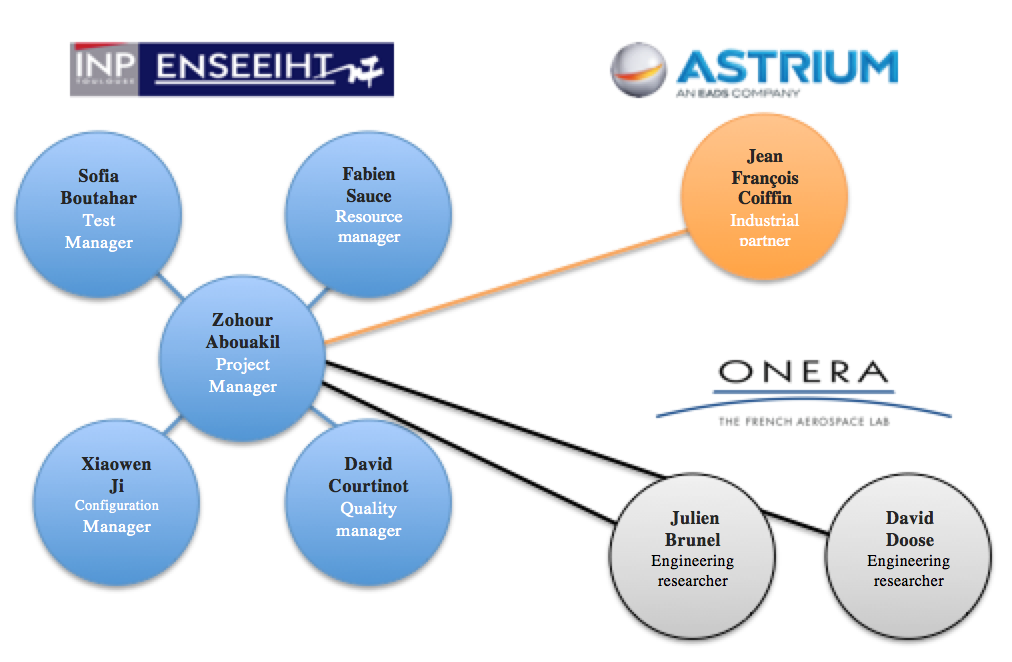
\includegraphics[scale=0.65]{data/teamOrganization.png}
~\\~\\Figure II.1 - The team organization of our project
\end{center}

\paragraph{}
\hspace{4mm}Although everybody was involved in the same manner in searching, coding and testing stages, we gave everyone a role in
order to improve the team organization. 
The project manager (Zohour \textsc{Abouakil}) had several responsabilities 
related to the project management. She has been in charge of the
communication with the industrial coordinator, Mr. Jean Francois
\textsc{Coiffin} and the scheduling of the different appointments.
David \textsc{Courtinot} was our quality manager and most of the time technical supervisor thanks to his knowledge of Scala
prior to the project.
Fabien \textsc{Sauce} was in charge of documenting the source code and reacting most of the meeting minutes.
Sofia \textsc{Boutahar} 
was responsible for the unitary tests and the regressions tests when 
there is a new version of the code or a part that is fully developped.
Xiaowen was in charge of the version tool Git and took care of the configuration of the few tools we used in the Project.

\paragraph{}
\hspace{4mm}In addition to being the project manager, Zohour established a 
contact with the client to see if the team is going in the right
direction or needed additional information.

\section{Project objectives in terms of management and organization}

\paragraph{}
\hspace{4mm}\begin{itemize} 
\item Managing coordination of the partners and working groups 
involved in the project.
\item Writing a detailed project planning including:
	\begin{itemize} 
	\item developing and maintaining a detailed development
	 plan.
	\item managing project deliverables in line with the 
	development plan.
	\item recording and managing project issues and escalating where
	 necessary.
	\item resolving issues and try to prevent them.
	\end{itemize}
\item Managing project scope and change control and escalating issues where necessary.
\item Monitoring project progress and performance.
\item Managing project evaluation and dissemination activities.
\item Final approval of the design specification.
\item Working closely with clients to ensure the project meets business needs.
\item Definition and management of the testing program.
\end{itemize}

\section{Deliverable documents}

\subsection{Delivrable documents expected by ENSEEIHT and the industrial supervisor}

\vspace{1.5mm}
\begin{itemize}
\item Report in PDF format\vspace{1mm}
\item Development plan in PDF format\vspace{1mm}
\item Presentation supports\vspace{1mm}
\end{itemize}

\subsection{Delivrable documents expected by the client}

\vspace{1.5mm}
\begin{itemize}
\item Documented source code in Scala language\vspace{1mm}
\item Test strategy\vspace{1mm}
\item Architecture design document\vspace{1mm}
\end{itemize}

\section{Development plan}

\subsection{Development organization}

\paragraph{}
\hspace{4mm}We used the Scrum method, which is widely used, 
and recognized for its efficiency. At first, 
we defined a product backlog containing all desired 
functionalities in the final product. Next, we divided the project into three
 << sprints >>(or << iterations >>). A sprint backlog is defined for 
each sprint, including all we need to realize at the end of an 
iteration. Each sprint lasts two weeks and consists in improving the 
software incrementally, to gradually become closer to the product backlog. 
At the end of each sprint, we organised a meeting, in order to 
review the progress and propose improvements or modifications
 of planning, but in the process of a sprint, the sprint backlog cannot be modified.
 To finish, each day started with a scrum meeting where each team member presented his objective of the day
 and his current difficulties, if any.

\subsection{Team organization approach for coding}

\paragraph{}
\hspace{4mm}We used an approach inspired by the XP (\textsc{extreme programming})
 method which is a practice of pair programming. Considering the amount of 
code that we had to write,
 we found it unnecessary that the five team members work separately,
 and we considered as excellent to work in pairs, in order to prevent 
errors and bias of the program structure, so that we can save precious time
 in testing and debugging. As a consequence, four of us worked
 in pairs and the last one works individually or supervises us. The groups repartition 
could change as the tasks were completed.

\subsection{Tasks organization}

\subsubsection{Task definition}

\paragraph{}
\hspace{4mm}The sprint backlog is a list of tasks that are identified by the members
 of the project and that has to be completed during the Scrum sprint.
During our meetings, we tried to estimate how many hours and
development efforts were needed to complete a task.

\paragraph{}
\hspace{4mm}\textbf{Sprint 1 backlog :}

\vspace{1.5mm}
\begin{itemize}
\item AST parsing of procedure C++ code\vspace{1mm}
\item CFG conversion from parsed AST\vspace{1mm}
\item Model checking with simple properties\vspace{1mm}
\end{itemize}

\paragraph{}
\hspace{4mm}\textbf{Sprint 2 backlog :}

\vspace{1.5mm}
\begin{itemize}
\item AST parsing of object oriented C++ code\vspace{1mm}
\item CFG conversion from parsed AST\vspace{1mm}
\item Model checking with simple criteria\vspace{1mm}
\end{itemize}

\paragraph{}
\hspace{4mm}\textbf{Sprint 3 backlog :}

\vspace{1.5mm}
\begin{itemize}
\item Improved CFG conversion from parsed AST\vspace{1mm}
\item Model checking with complex criteria\vspace{1mm}
\end{itemize}

\subsubsection{Task planning}

\paragraph{}
\hspace{4mm}Our sprint backlog was maintained as a spreadsheet. 
During the Scrum sprint, each team member was requested to 
keep the sprint backlog updated.

\section{Risk management}

\subsection{Risk management strategy}

\paragraph{}
\hspace{4mm}The first step in project risk management is to identify the risks
 that may arise during the project. Some risks have a higher impact than others, 
and are more or less likely to occur. Basing on those two criterias, we classified the risks
in order to visualize which points we had to focus on in priority to avoid problems in the future.

\subsection{Risk analysis}

\paragraph{}
\hspace{4mm}Below is a table that summarizes the major risks that we could face in our project and how we planned to prevent them.

\begin{center}
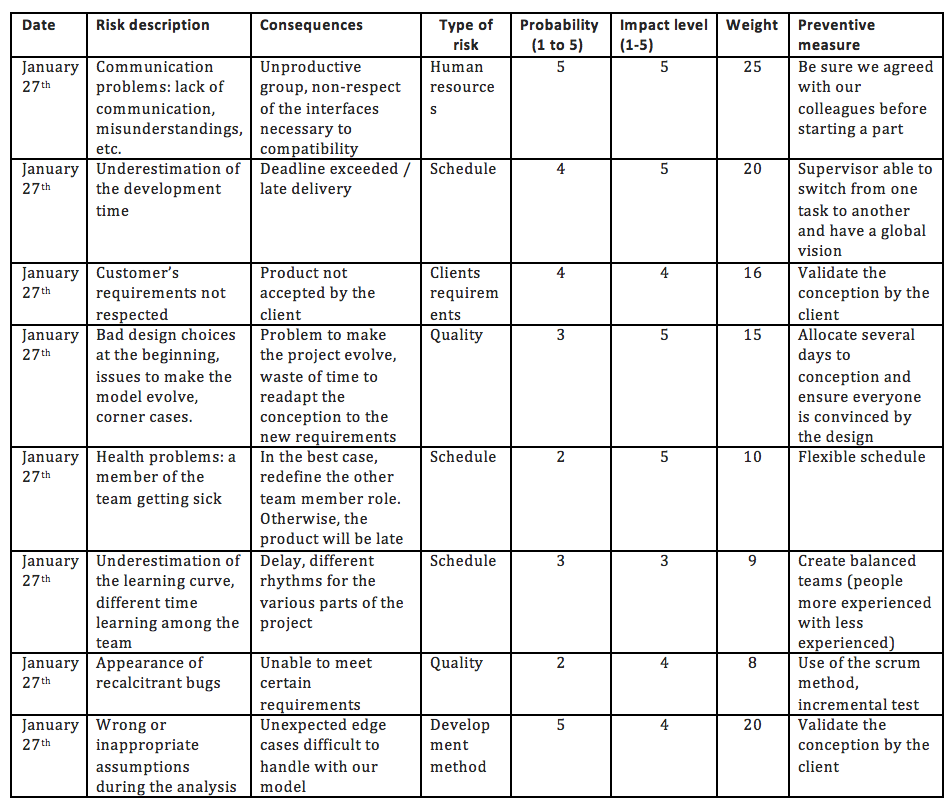
\includegraphics[scale=1.0]{data/RiskManagement.png}
~\\~\\Figure II.2 - The risk analysis for our project
\end{center}

\section{Resource management system}

\subsection{Versioning tool}

\paragraph{}
\hspace{4mm}We used Git to manage our project, more particularly the versioning of the code
and the documents that we redacted. We chose Git because it is a free and open-source
 distributed version control system that handles any software 
project in a highly efficient way. It also supports rapid branching and merging, 
and includes specific tools for visualizing and 
navigating through the development history.
All the delivrable documents were managed on a git repository, including documentation and reports. 
Anyone was allowed to commit at anytime, however any push had to be authorized by the quality responsible after the code has been thoroughly tested against a 
set of tests by the test responsible.

\subsection{Communication between team members}

\paragraph{}
\hspace{4mm}We used Google Drive to share all the documents 
between the team members.
 In particular, we stored on the drive the following contents :
all the research papers and the interesting documents
 that we found or were given by the clients, pointers to external documentation,
all documents related to the project management (planning, current sprint backlog...),
minutes of the meetings either with 
the clients or the industrial coordinator.

\section{Code and documentation}

\subsection{Quality checking}

\paragraph{}
\hspace{4mm}For ensuring that our coding rules were respected and
 evaluating the quality of our sources,
 we used a tool called Scalastyle that enables, using an easy-to-use xml configuration file,
 to examine the scala code and indicates potential problems with it.
 Combined with a specific pulgin, this can be used to generate 
warnings or errors in the IDE the developer is using. 
Our settings were the following :

\definecolor{mygray}{gray}{0.4}
\renewcommand{\arraystretch}{1.2}
\begin{center}
\begin{longtable}{|l|l|l|}
\hline
\textbf{\textcolor{mygray}{Rule}} & \textbf{\textcolor{mygray}{Description}} & \textbf{\textcolor{mygray}{Value}}  \\
\hline
FileLengthChecker & \small{Check the number of lines in a file} & 1500  \\
\hline
FileLineLengthChecker & \small{Check the number of characters in a line} & 140 \\
\hline
FileTabChecker & \small{Check that there are no tabs in a file} & enabled \\
\hline
ClassNamesChecker & \small{Check that class names match a regular}  & \^ [A-Z][A-a-z]*\$ \\
& \small{expression} & \\
\hline
\small{ClassTypeParameterChecker} & \small{Checks that type parameter to a class matches a} & \^[A-Z\_]\$ \\
& regular expression & \\
\hline
FileTabChecker & \small{Check that there are no tabs in a file} & enabled \\
\hline
\small{CyclomaticComplexityChecker} & \small{Checks that the cyclomatic complexity of a method} & 12 \\
&  \small{does exceed a value} & \\
\hline
EmptyClassChecker & \small{If a class/trait has no members, the braces are} & enabled \\
&  \small{unnecessary} & \\
\hline
\small{EqualsHashCodeChecker} & \small{Check that if a class implements either equals} & enabled \\ 
 & \small{or hashCode, it should implement the other} & \\
\hline
MethodLengthChecker & \small{Checks that methods do not exceed a maximum} & 50 \\
& \small{length} & \\
\hline
MethodNamesChecker & \small{Check that method names match a regular} & \^[a-z][A-Za-z0-9]*(\_=)?\$ \\
\tiny{.} & \small{expression} & \\
\hline
\small{MultipleStringLiteralsChecker} & \small{Checks that a string literal does not appear} & allowed = 2 \\
& \small{multiple times} & \\
\hline
\small{NotImplementedErrorUsage} & \small{Checks that the code does not have ??? operators} & enabled \\
\hline
NullChecker & \small{Check that null is not used} & enabled \\
\hline
\small{NumberOfMethodsInTypeChecker} & \small{Check that a class/trait/object does not have too} & maxMethods = 30 \\
& \small{many methods} & \\
\hline
NumberOfTypesChecker & \small{Checks that there are not too many types} & maxTypes = 20 \\
& \small{declared in a file} & \\
\hline
ObjectNamesChecker & \small{Check that object names match a regular}  & \^[A-Z][A-Za-z]*\$ \\
& \small{expression} & \\
\hline
ParameterNumberChecker & \small{Maximum number of parameters for a method} & maxParameters = 5 \\
\hline
RedundantIfChecker & \small{Checks that if expressions are not redundant, ie} & enabled \\
& \small{easily replaced by a variant of the condition} &  \\
\hline
ScalaDocChecker & \small{Checks that the ScalaDoc on documentable}  & enabled \\
& \small{members is well-formed} & \\
\hline
\end{longtable} 
\end{center}
\paragraph{}
\hspace{4mm}This project meets a need from our clients. 
Therefore our codes will probably be used, studied and modified. 
That is why we have set up this quality approach. 
All our codes should be understandable and well commented. 
To achieve that, our programs were constantly reviewed by our clients
as we gave them the link to our Git repository.

\subsection{Verification and validation process}

\subsubsection{Verification}

\paragraph{}
\hspace{4mm}Verification is the process in which we determine
whether the right solution is being developed.
Once a functionality of our product is completed, 
we analyze the results in order to
 verify that the requirements have been met. 
 In addition, the verification is an ongoing process:
 at the each completion of each milestone, 
we performed a verification analysis to make 
sure we were still on track.

\paragraph{}
\hspace{4mm}As we have chosen the \textsc{Extreme Programming} model for the programming 
aspect of the project, we considered that a code passes
 the quality test if at least the two members of a pair have checked 
it. This is up to the quality manager to ensure this has been done, 
otherwise he should do it himself. This was specific to the code quality 
checks and did not apply to the rest of the delivrable documents.

\subsubsection{Validation}

\paragraph{}
\hspace{4mm}Validation is the process in which we make sure that the solution
that we came up with is 
constructed correctly and according to the requirements 
and the specifications.
In this process, we performed various testing procedures on
 the code and tried to remove the defects as soon as possible. 
Once the found defects have being fixed, the process repeated itself.

\chapter{Technical aspects}

\section{Context}

\subsection{Motivations}

\paragraph{}
\hspace{4mm}As a reminder, the aim of the project was to assert some good properties on embedded systems source code written in C++. More precisely,
it consisted in static analysis of C++ programs. Thus, some properties cannot be checked by our software as they require runtime analysis.
Nevertheless, a well-written code is more likely to work well, making such a tool interesting for checking the quality of a C++ source code.

\subsection{Objectives}

\paragraph{}
\hspace{4mm}The model checking, which consists in asserting properties 
on a model thanks to graph search algorithms (for example),
 is one of those fields that can be applied to this matter.
 In this project, we were trying to build a model checker working
 on C++ code which takes the source code as an input and is 
transformed a few times in various abstract representations to end 
with a graph model that we are able to send to a model checker.

\section{Definitions}

\subsection{The AST - Abstract Syntax Tree}

\paragraph{}
\hspace{4mm}The \textsc{AST} is an abstract (and low-level) representation of the 
abstract  syntactic structure of the source code.
It is a tree data-structure which describes the code in a purely 
syntactic point of view. Each node of the tree denotes a
 construct occurring in the source code. The syntax is "abstract" 
because it's not representing  every detail appearing in the real syntax. 
However, the \textsc{AST} can contain additional data as the position of 
an element in the source code node.
You can see below a
 simple \textsc{C/C++} code and its AST representation. 
The \textsc{AST} is provided by the Clang API, which performs the first step
 of our transformation chain.

\begin{lstlisting}[language=java]
int main() {
    int a = 5;
    if (a > 6) {
        int c = 5;
        c *= 5;
    }
    int b = 17;
}
\end{lstlisting}
\begin{center}
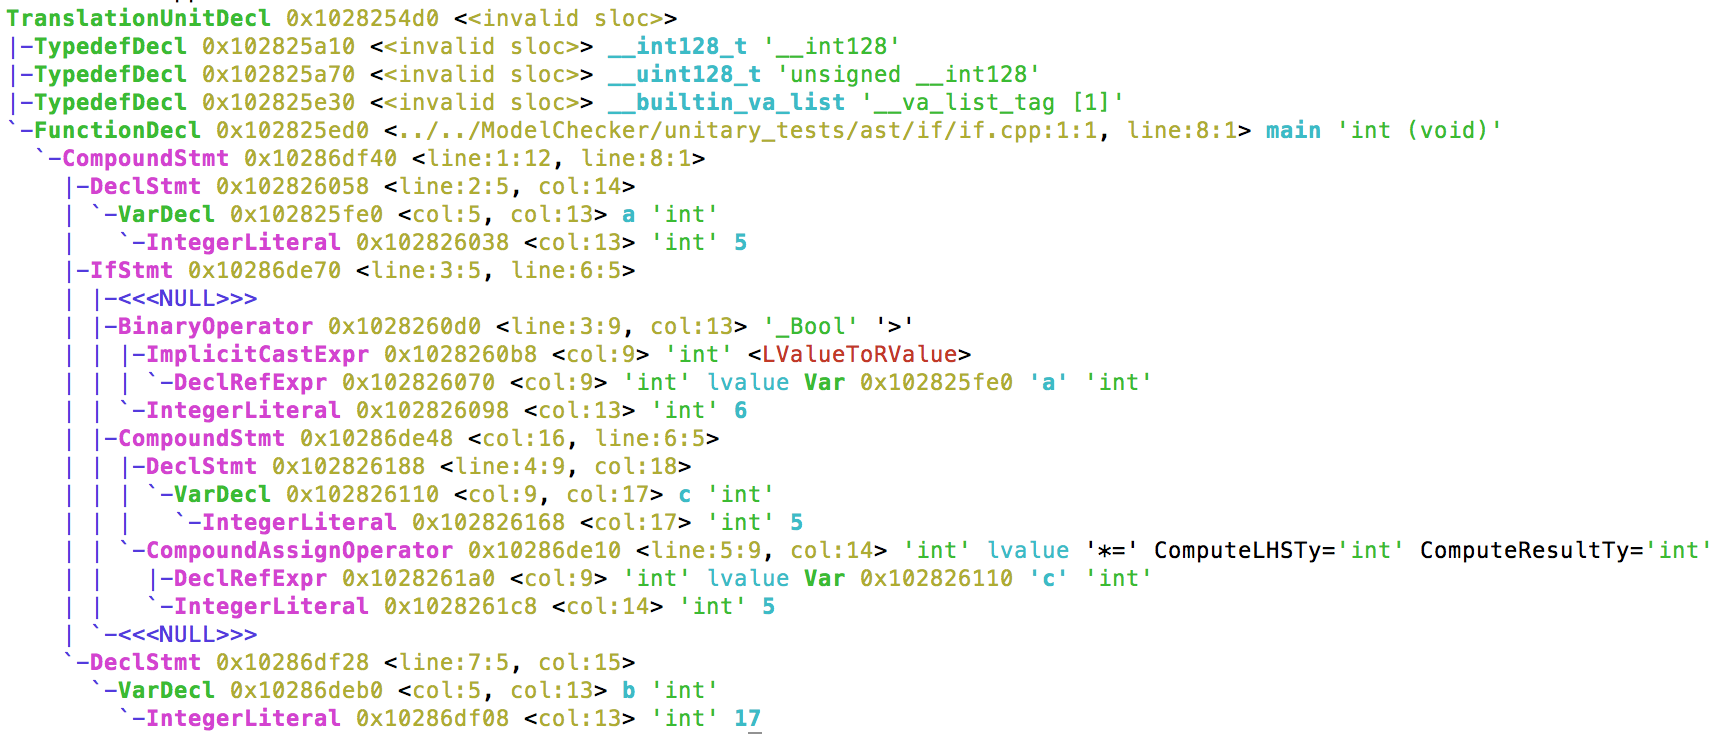
\includegraphics[scale=0.6]{data/ifClang.png}
~\\~\\Figure III.1 - The AST of the C++ code generated by the clang API
\end{center}

\paragraph{}
\hspace{4mm}\definecolor{oliveGreen}{RGB}{0,102,0}
The indentation in the AST is the depth of a node. Nodes that have
the same level of indentation are brothers. Each node can have 
children that are separated by a new line and a \textcolor{blue}{|\_}. 
We should notice
that the last child of a node starts it's representative line by \textcolor{blue}{`\_}
.  For example the \textcolor{oliveGreen}{TranslationUnitDecl} has four children :
the first three childs are \textcolor{oliveGreen}{TypedefDef} and
 the last one is a \textcolor{oliveGreen}{FunctionDecl}.
To traverse the full AST, we start from the \textcolor{oliveGreen}{TranslationUnitDecl}
 and then recursively traverse everything 
that can be reached from that node
The toplevel declaration in a translation unit is always the
 translation unit declaration. 
In this example, our first user written declaration 
is the declaration of the function "main" that contains
a declaration of the variable a and then an If statement.
The \textcolor{magenta}{IfStmt} (if statement) has a condition and a body. The condition is 
described in this example by the binary operator \textcolor{blue}{>} that has two
childs which are the operands \textcolor{blue}{a} and \textcolor{blue}{6}. 
The body of the \textcolor{magenta}{IfStmt} is described by the compound statement which is 
a combination of two or more simple statements. In this case, it's 
a combination of a \textcolor{magenta}{declStmt} (declaration statement) in which the declaration and 
initialization of  the variable \textcolor{blue}{c} to \textcolor{blue}{5} 
is described and a compoundAssignOperator 
in which the assignment operation is described.
In the end, there is a \textcolor{magenta}{DeclStmt} that describes the declaration and initialization
of the variable \textcolor{blue}{b} to \textcolor{blue}{17}.

\subsection{CFG - Control Flow Graph}

\paragraph{}
\hspace{4mm}A control flow graph \textsc{CFG} is a graph representation of 
all paths that might be traversed through a program during 
its execution. We do have some restrictions, 
for example we won't create several nodes for a single expression 
even if in reality an expression should be a graph. This is shown 
in the example below.

\begin{center}
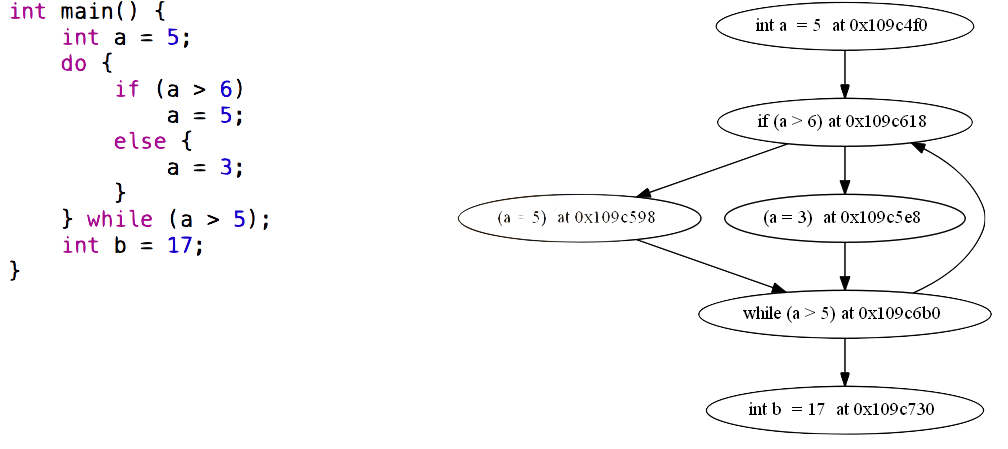
\includegraphics[scale=0.8]{data/codeCFG.png}
~\\~\\Figure III.2 - An example of a CFG (a doWhile block here)
\end{center}

\paragraph{}
\hspace{4mm}We can clearly see in the example above the
CFG representing all the possible execution paths of the C/C++ program.

\subsection{CTL - Computation Tree Logic}

\paragraph{}
\hspace{4mm}CTL is a way of representing temporal logic expressions on a graph or a tree. For example, it can
express properties such as \textit{<< All the paths starting from every node verifies the predicate p >>}.

\section{\textsc{AST} and \textsc{CFG} representations}

\paragraph{}
\hspace{4mm}After studying the Clang API, we came to the conclusion that the
 AST is a much more low-level representation of the program than
 the CFG. 
Indeed, the atom for a CFG is what is generally called a 
\textit{statement}, whereas the simplest instruction is represented by an AST 
composed of multiple nodes. In addition, we found it 
difficult to handle the parsing/creating and the linking of the graph nodes at 
the same time.
Thus, we have chosen to transform the original AST nodes into a serie of 
higher-level objects, which will be converted into nodes of the CFG.

\paragraph{}
\hspace{4mm}In order to create a GraphNode, we had to follow the steps shown 
in the figure below.

\begin{center}
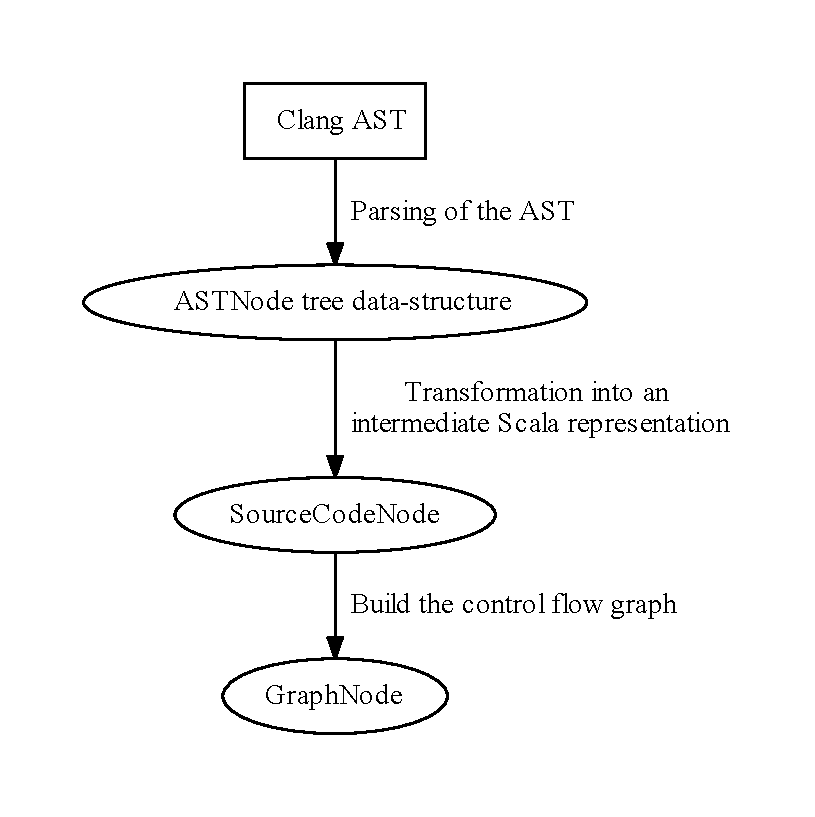
\includegraphics[scale=0.65]{data/transform_chain}
~\\~\\Figure III.3 - Transformation chain
\end{center}

\subsection{Parsing the clang AST File}

\paragraph{}
\hspace{4mm}At first, 
we considered using XML parsing libraries to parse 
the XML version of the Clang AST. 
However, this type of output is no longer supported by the newest
 versions of the Clang compiler and all the existing tools
provide partial support at best. Hence, we decided to use the
 regular AST file and parse it line by line with a custom parser.

\paragraph{}
\hspace{4mm}We identified three main types of nodes in the AST. 
Each one is associated to a specific class which extends ASTNode.

\vspace{1.5mm}
\begin{itemize}
\item Nodes consist of a type name, an id, a code pointer pointing 
the relevant lines of the code and some metadata that depend on
 the type of the node. These are represented by the 
\textbf{ConcreteASTNode class}.\vspace{1mm}
\item \textbf{< < <NULL> > >} children, represented by the \textbf{NullASTNode} class.\vspace{1mm}
\item Other kind of nodes, prior to class declaration for example.
 These are represented by \textbf{OtherASTNode}.\vspace{1mm}
\end{itemize}

\paragraph{}
\hspace{4mm}The file is parsed and converted in a tree data-structure 
which nodes are of type ASTNode. 
The ASTNode objects will then be converted in Stmt or Decl 
accordingly to the class hierarchy we present in the next part.

\begin{center}
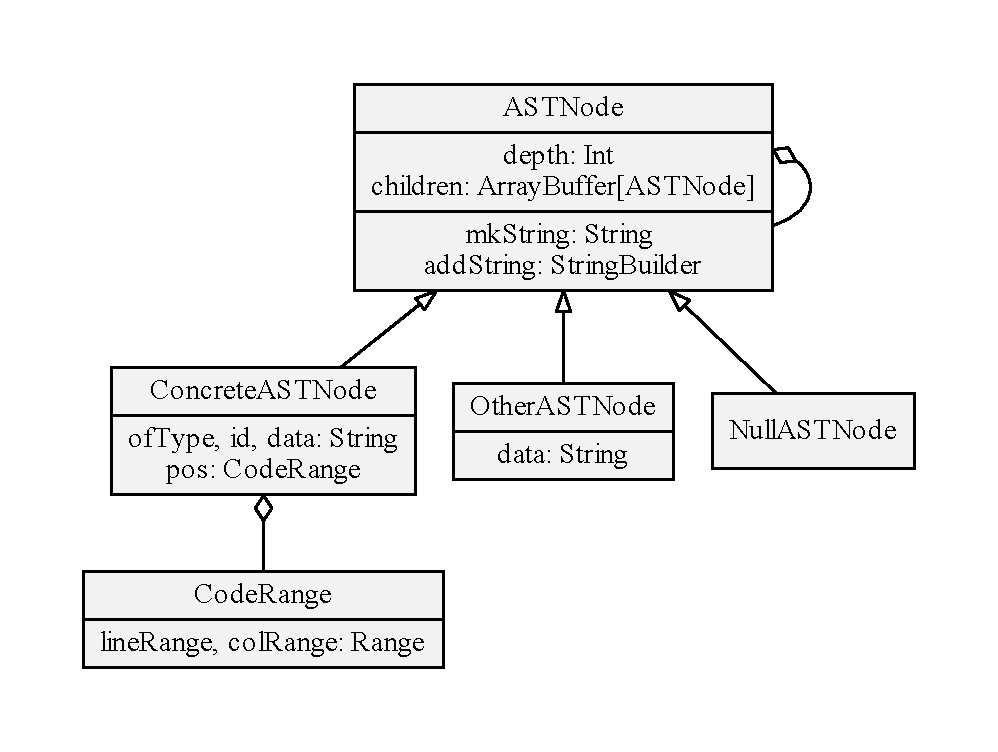
\includegraphics[scale=0.6]{data/AST_classes}
~\\~\\Figure III.4 - Class hierarchy for the output format of the ASTParser
\end{center}

\subsection{From ASTNode to SourceCodeNode}

\paragraph{}
\hspace{4mm}The \textbf{SourceCodeNode} class represents a tree data-structure
 which is still close enough to the AST but with a higher abstraction
 and some removed low-level information.

\section{Model checking}

\paragraph{}
\hspace{4mm}The biggest problem we ran into in this part was to achieved a high level of genericity while keeping
a simple architecture, not overly complicated to use for a specific case. We also had to ensure that the architecture is
free of any dependance of any kind with the CFG part.

\paragraph{}
\hspace{4mm}We have identified three kind of entities involved in model checking, each of them corresponds to a generic type :

\vspace{1.5mm}
\begin{itemize}
\item a type M describing the meta-variables. M must extend the MetaVariable trait.\vspace{1mm}
\item a type N describing the values contained by the nodes of the graph (GraphNode[N]). N can be anything.\vspace{1mm}
\item a type V describing the values of the environment. V must extend the Value trait\vspace{1mm}
\end{itemize}

\paragraph{}
\hspace{4mm}One could wonder why we chose using (M <: MetaVariable,V <: Value) instead of 
just (M,V) or (MetaVariable,Value). Here are the advantages of the proposed solution compared to the two others :

\vspace{1.5mm}
\begin{itemize}
\item \textbf{(M <: MetaVariable,V <: Value) vs (M,V)} : more evolutive, we can imagine adding
operations on MetaVariable and Value in the future. This is an advantage for developing new features on the CTL part.\vspace{1mm}
\item \textbf{(M <: MetaVariable,V <: Value) vs (MetaVariable,Value)} : more accurate type. This enables the developer using the model checker to
specialize these generic classes in a more powerful way than it would be in the second case, because the access to specific methods of M and V would be lost.
This is an advantage for using the CTL part in any kind of application.\vspace{1mm}
\end{itemize}

\subsection{Representation of the environments}

\paragraph{Definition 1}
A \textit{positive binding} is an element of $M \times V$. It associates a meta-variable to a specific value.

\paragraph{Definition 2}
A \textit{negative binding} is an element of $M \times \mathscr{P}(V)$. It associates a meta-variable to a set of illegal values.

\paragraph{Definition 3}
Two bindings are said \textit{in conflict} if :

\vspace{1.5mm}
\begin{itemize}
\item they are two positive bindings $(m,v_1)$ and $(m,v_2)$ such as $v_1 \neq v_2$\vspace{1mm}
\item they are one positive binding $(m,v)$ and one negative binding $(m,V)$ such as
$v \in V$\vspace{1mm}
\end{itemize}

\paragraph{Definition 4}
An \textit{environment} is a set of positive and negative bindings.  An environment 
containing conflicting bindings is noted $\bot$.

\subsection* {Methods and class hierarchy}
\paragraph{}
\hspace{4mm}At first, positive and negative bindings were stored in two separate maps but we finally decided 
to use an abstract class MetaVarBinding extended by two case-classes to represent all kinds of bindings and use a single map.
The Environment class contains all the abstract operations between or on environments required by the algorithm :

\vspace{1.5mm}
\begin{itemize}
\item intersection (noted \& in reference to the \& method of the Set trait)\vspace{1mm}
\item removal of a binding (noted - as it is a standard notation for removal in a Scala collection)\vspace{1mm}
\item opposite (noted ! in reference to the logical negation in Scala)\vspace{1mm}
\end{itemize}

\paragraph{}
\hspace{4mm}The following diagram presents the chosen design for environments. Next parts of this section will focus on explaining it all :

\begin{center}
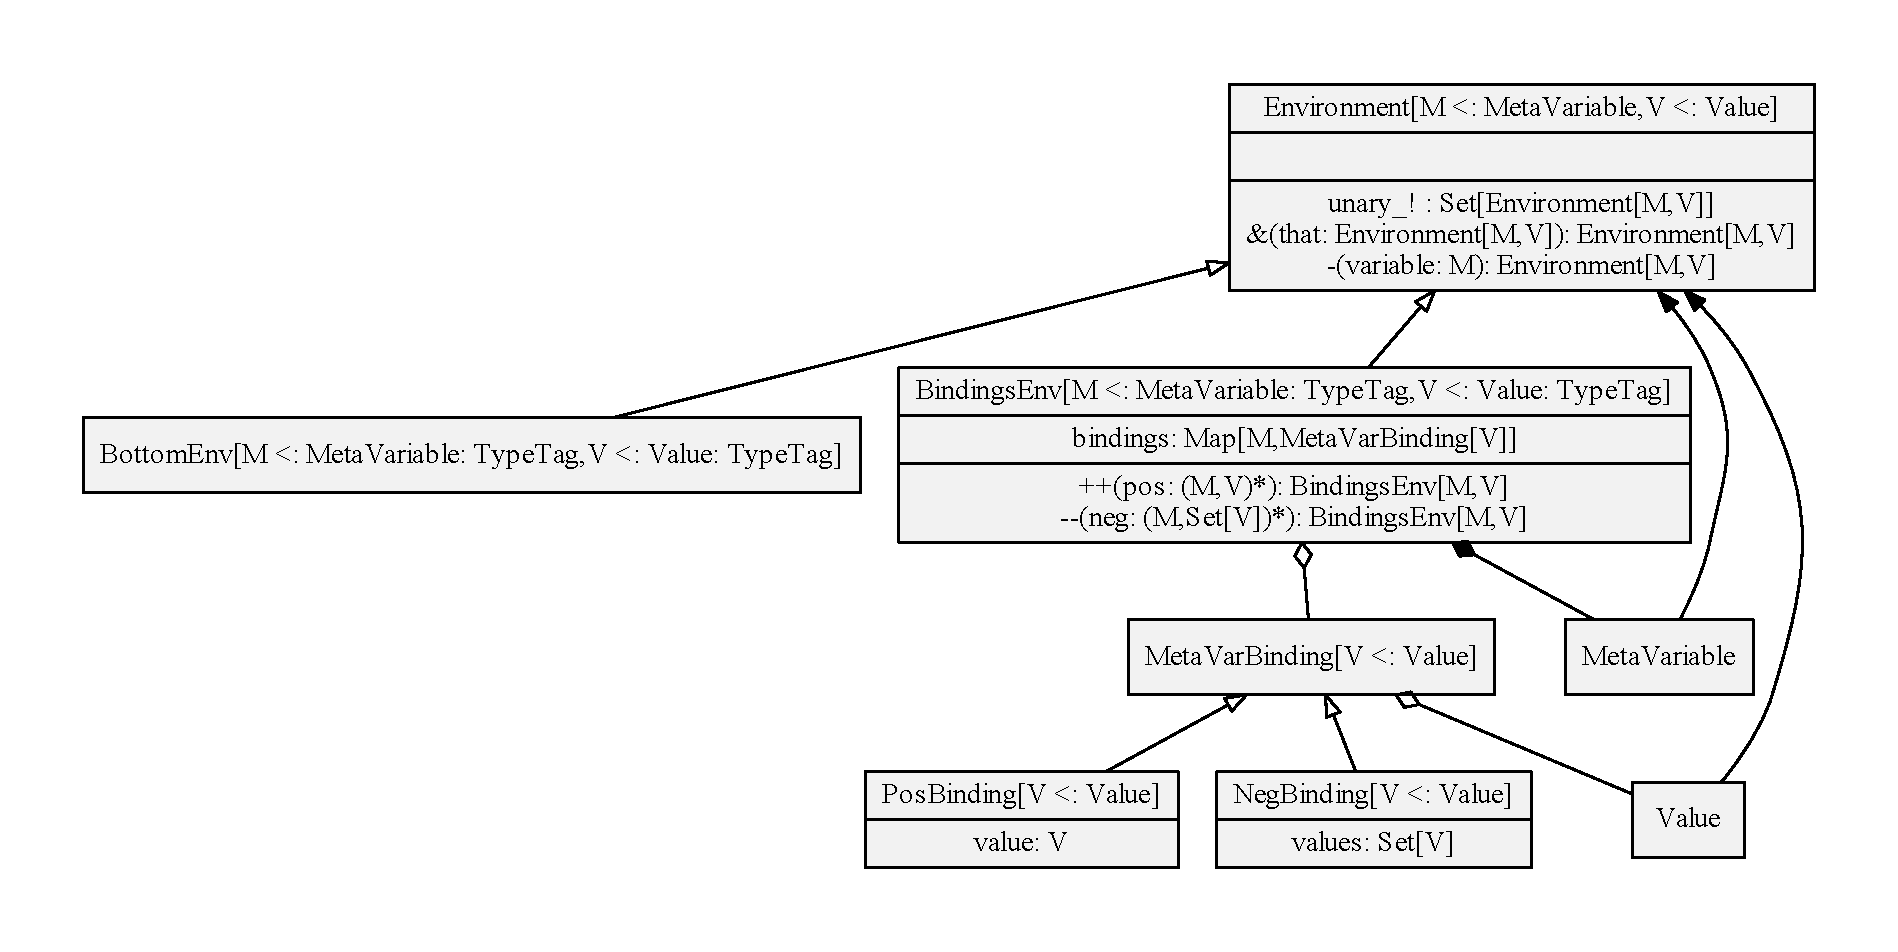
\includegraphics[scale=0.5]{data/Env}
~\\~\\Figure III.5 - Environement class hierarchy
\end{center}

\subsection* {The specific case of the $\bot$ environment}
\paragraph{}
\hspace{4mm}The $\bot$ environment was a bit tricky to represent. Indeed, environments depend on generic types
M and V, which implies that Environment must be a generic class. Thus, BottomEnv also must to be generic. However, 
considering the mathematical definition of $\bot$, it would be poor design to represent it with a regular class instead of a singleton.

\paragraph{}
\hspace{4mm}We want all self-contradictory environment of the same generic type to be equal, and if possible we would like two self-contradictory environments of
different generic types not being equal, to keep the type consistency. As Scala does not allow a singleton to be generic (which is quite logical by the way=,
we have had to use reflexivity to implement the singleton pattern without using the \textbf{object} keyword. We also used some implicit definitions to allow nice syntax using 
the Bottom object to fetch the BottomEnv singleton of the appropriate type given the context.

\subsection* {Regular environments}
\paragraph{}
\hspace{4mm}Having defined the MetaVarBinding class and its children case-classes, it seems natural to use a single Map[M,MetaVarBinding[V]] map to
represent the bindings. The only real design problem we have got here was the fact that the reflexivity used to solve the BottomEnv problem
was infectious. We have had to use TypeTag(s) in some generic methods and in the BindingsEnv constructor. Thus, any external code
calling the main constructor was forced using TypeTag(s) also. To address this issue, we made the main constructor private and declared and secondary constructor
TypeTag-free creating an empty BindingsEnv object. The user then has to add bindings to this environment using the ++ and - - methods.

\subsection{CTL expressions}

\subsection* {Defining the CTL-V language}
\paragraph{}
\hspace{4mm}There is nothing too difficult here, the class hierarchy is directly derived from the mathematical
definition of CTL operators. The only interesting points are the way of defining generic predicates as well as the way of quantifying variable with the $\exists$ quantifier. These points
will be discussed in the next subsections. Another thing to mention is that we did not define AG, EG, AF and EF as classes but used the mathematical equivalences between the different operators
to define them with implicit declarations using the other operators. This way, we don't have to handle them as particular cases in the model checking algorithm since they are first converted into
a combination of the other operators.

\begin{center}
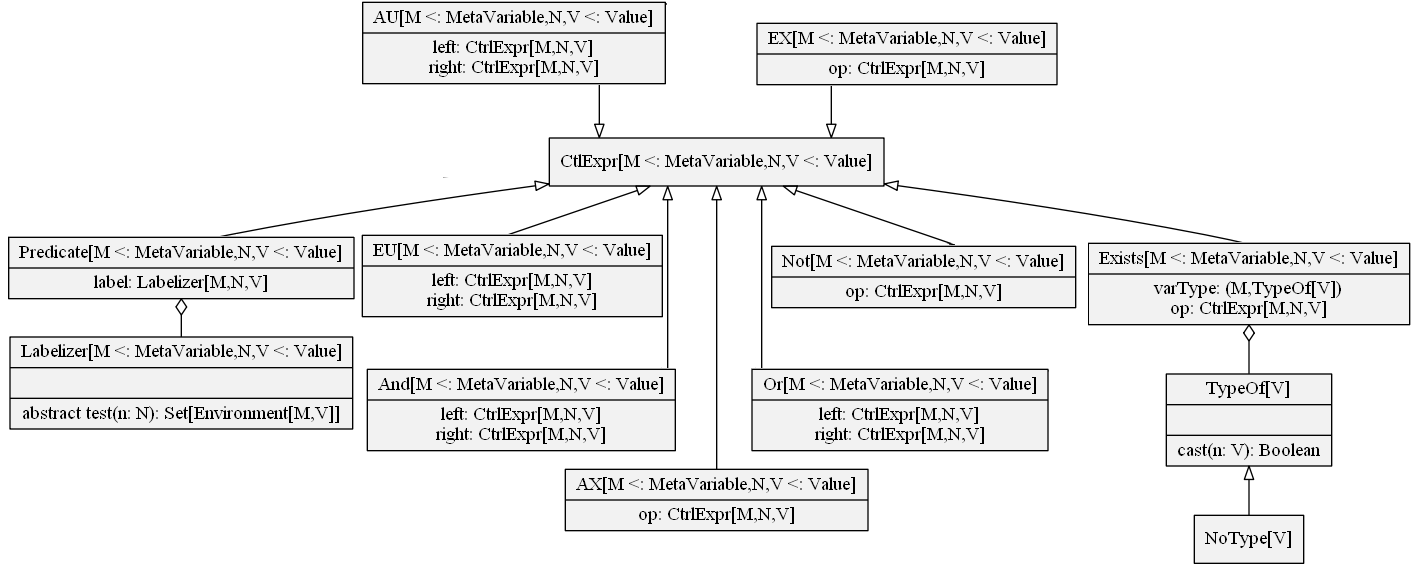
\includegraphics[scale=0.4]{data/CTL_expr.png}
~\\~\\Figure III.6 - CTL expression class hierarchy
\end{center}

\subsection* {Predicates}
\paragraph{}
\hspace{4mm}To enable to make generic predicates, we simply defined a generic class Predicate that wraps a Labelizer. A Labelizer
defines a \textit{test} method that takes an object of type N (the type of the GraphNode(s)) and returns an Option[Environment[M,V]].
If the predicate is not verified by the input node, this method must return None, otherwise it returns the set of positive bindings that make the node
match the predicate. This set is possibly empty if the predicate does not involve any meta-variable.

\subsection* {$\exists$ quantifier}
\paragraph{}
\hspace{4mm}The $\exists$ quantifier is a bit tricky to define because of the ex\_binding operation defined in the model checking algorithm, which requires
to know the set of all possible values for a given meta-variable. The problem is that the type V may be composed of inconsistent types wrapped by some classes extending V. For example, in the case of the model checking on the CFG,
if X has been assigned a negative binding composed of declarations, then we should not consider that X could possibly be an Expr.

\paragraph{}
\hspace{4mm}To sum up, we must be able to have a type information about the meta-variable at least when encountering the $\exists$ quantifier. Therefore
we introduced the TypeOf class which defines a cast operation. This way, incompatible values will be filtered. This is completely generic as the cast operation is defined by the user depending on its needs.

\subsection{Model checker}

\paragraph{}
\hspace{4mm}The only interesting thing to mention here is the use of a conversion method for compute the Val set of all possible values.
In order to compute Val, all the nodes of the graph are traversed. For each node, we call the converter that returns all the values of type V a given node is likely to add to the environment. Note that 
a single node can introduce several values in the environment (for example a node f(5,6) would inject 5 and 6 when applying a f(x,y) labelizer), that's why the converter must return a Set[V]. We could have defined
the conversion as an abstract method of the GraphNode, but we thought it was more convenient to do it externally. It is exactly the same difference as
Comparable and Comparator in Java : Comparable defines the comparison operation directly on the class, it is useful when a natural order exists but it enables only one implementation
of the comparison whereas we can define as many Comparator(s) as we want for the same type.

\section{Merge}

\subsection{Choice of M, N and V}

\paragraph{}
\hspace{4mm}Considering the kind of predicates we wanted to use and the types of node we were using (as a recall, type N will be ProgramNode for the CFG), it was kind
of obvious that we would need Expr values in our environment, so we introduced the type CFGExpr, which simply wraps an Expr object. However, it was not so easy determining what other kinds
of values would be required. To solve this question, we thought about the labelizers and properties we wanted to be able to implement to deduce our needs. 
Two important properties led us to introduce types CFGDecl and CFGExpr :

\vspace{1.5mm}
\begin{itemize}
\item << \textit{There should be no hidden declarations  (declaration of an entity of the same kind, same type and same name in different scopes)} >>\vspace{1mm}
\item << \textit{There should be no declared entity which is never used} >>\vspace{1mm}
\end{itemize}

\paragraph{}
\hspace{4mm}We can see there that \textit{declaration} has a slightly different meaning in those two cases. In the first case,
two declarations are considered equal (this is the way we have to interpret \textit{hidden} in order to create conflicts in the environments in case
of hidden declarations) if they declare an entity of the same kind, type and 
name. We prefer calling that a \textit{definition} rather than a \textit{declaration}. In the second case,
all declarations have to be considered unique because we do not care if a variable of the same type and name corresponding to a declaration was used in the code,
we want to know if every declaration, individually, was used. Thus, CFGDef will be used to represent a definition, and CFGDecl to represent a declaration.
The only difference between those two is that CFGDecl takes an id as a parameter and bases its equality check on this id whereas CFGDef bases it on the pair (type,name).

\paragraph{}
\hspace{4mm}Finally, we saw that it could be interesting to make some type checks, or for example, when looking for arithmetic on pointers, which requires to distinguish the = operator, which is allowed for pointers, from + or -, which are deprecated).
Therefore, we also allowed strings to be values of the environment, so we created a wrapper type CFGString. The following diagram sums this all up :

\begin{center}
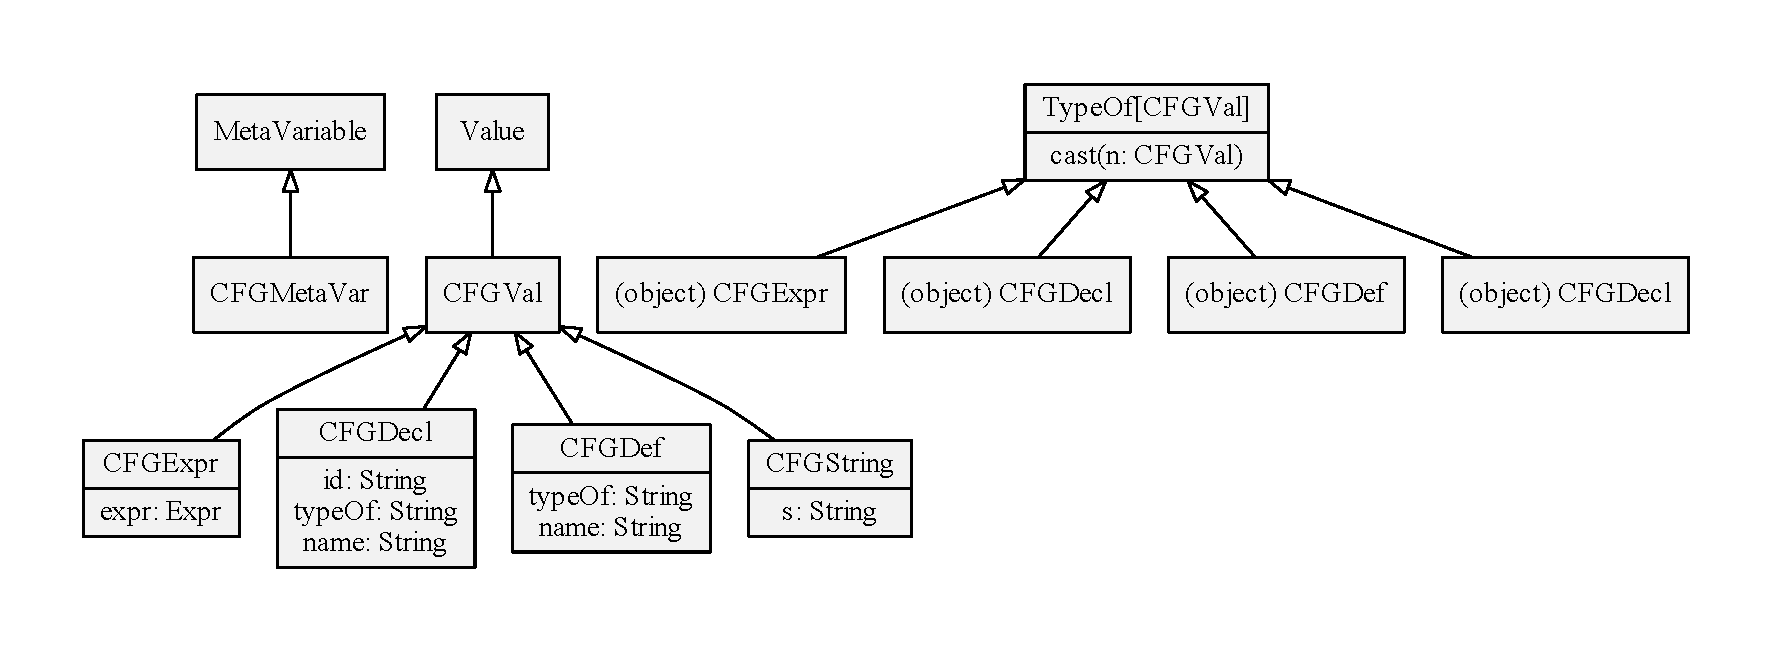
\includegraphics[scale=0.65]{data/merge_types}
~\\~\\Figure III.7 - Concrete implementation of the generic types of the CTL part
\end{center}

\subsection{Labelize our nodes}

\subsection* {Patterns}
\paragraph{}
\hspace{4mm}Most of the predicates we need to use were based on the idea of a pattern of code. For example, $X = 0$ is a pattern describing all the assignments to 0
of a variable to be determined (using capital-size letter means that this is a meta-variable and not a variable of the code). Using patterns, we are able 
to tell many things about a node and express many base properties. The patterns had to be able to match all kinds of entities in a code and allow for 
returning bindings between the meta-variables of the pattern and the matching values in case of success of the matching. For the same reasons as in the
previous part, we determined that we needed :

\vspace{1.5mm}
\begin{itemize}
\item patterns for expressions : ExprPattern\vspace{1mm}
\item patterns for declarations : DeclPattern\vspace{1mm}
\item patterns for string values : StringPattern\vspace{1mm}
\end{itemize}

\paragraph{}
\hspace{4mm}For expression patterns, we did not want to explore more than one level of depth of the expressions.
Deeper exploration of the expression tree would be nearly pointless for the properties we aim to assert on the CFG, moreover
some patterns may be ambiguous or more bothering to define if we explored the tree deeper (for example, $5 + x + y + 6$ can be matched in several ways by the $X + Y$ patterns, 
X and Y being meta-variables). Even if the AST generated by an expression is deterministic, which makes deep pattern matching possible, we thought it was not very clear for the user
what he would get when using deep patterns. Therefore, we introduced the AtomicExprPattern, which is only extended by leaves expressions patterns and is the only kind of ExprPattern
that can be passed as a parameter to a non-leave expression pattern. This choice is entirely reversible and has no consequence on the rest of our design.

\paragraph{}
\hspace{4mm}StringPattern and ExprPattern have in common the fact that they can be whether an UndefinedVar, which is a simple wrapper of a meta-variable that matches anything
and returns the appropriate binding, or a specific value (DefinedExpr, DefinedString). StringPattern can also be a NotString, which is comparable to a negative binding : it is a set
of forbidden values. We did not need to use such thing for ExprPatttern, but nothing in our conception prevents us from adding it later.

\paragraph{}
\hspace{4mm}Finally, DeclPattern is a bit different than the other two. It can also be an UndefinedVar, but we did not see any use-case for a DefinedDecl pattern. 
We actually only treated variable declarations, which required to have a powerful pattern-matching based on the name, the type and the assigned expression, if any.
We needed two patterns doing mostly the same thing but returning in one case a CFGDecl, and in the other case a CFGDef. Consequently, we factorized the code of those two patterns
in VarDeclMatcher. The specific behaviour of VarDefPattern and VarDeclPattern is implemented in the conversion method passed as a parameter in the constructor of VarDeclMatcher.

\begin{center}
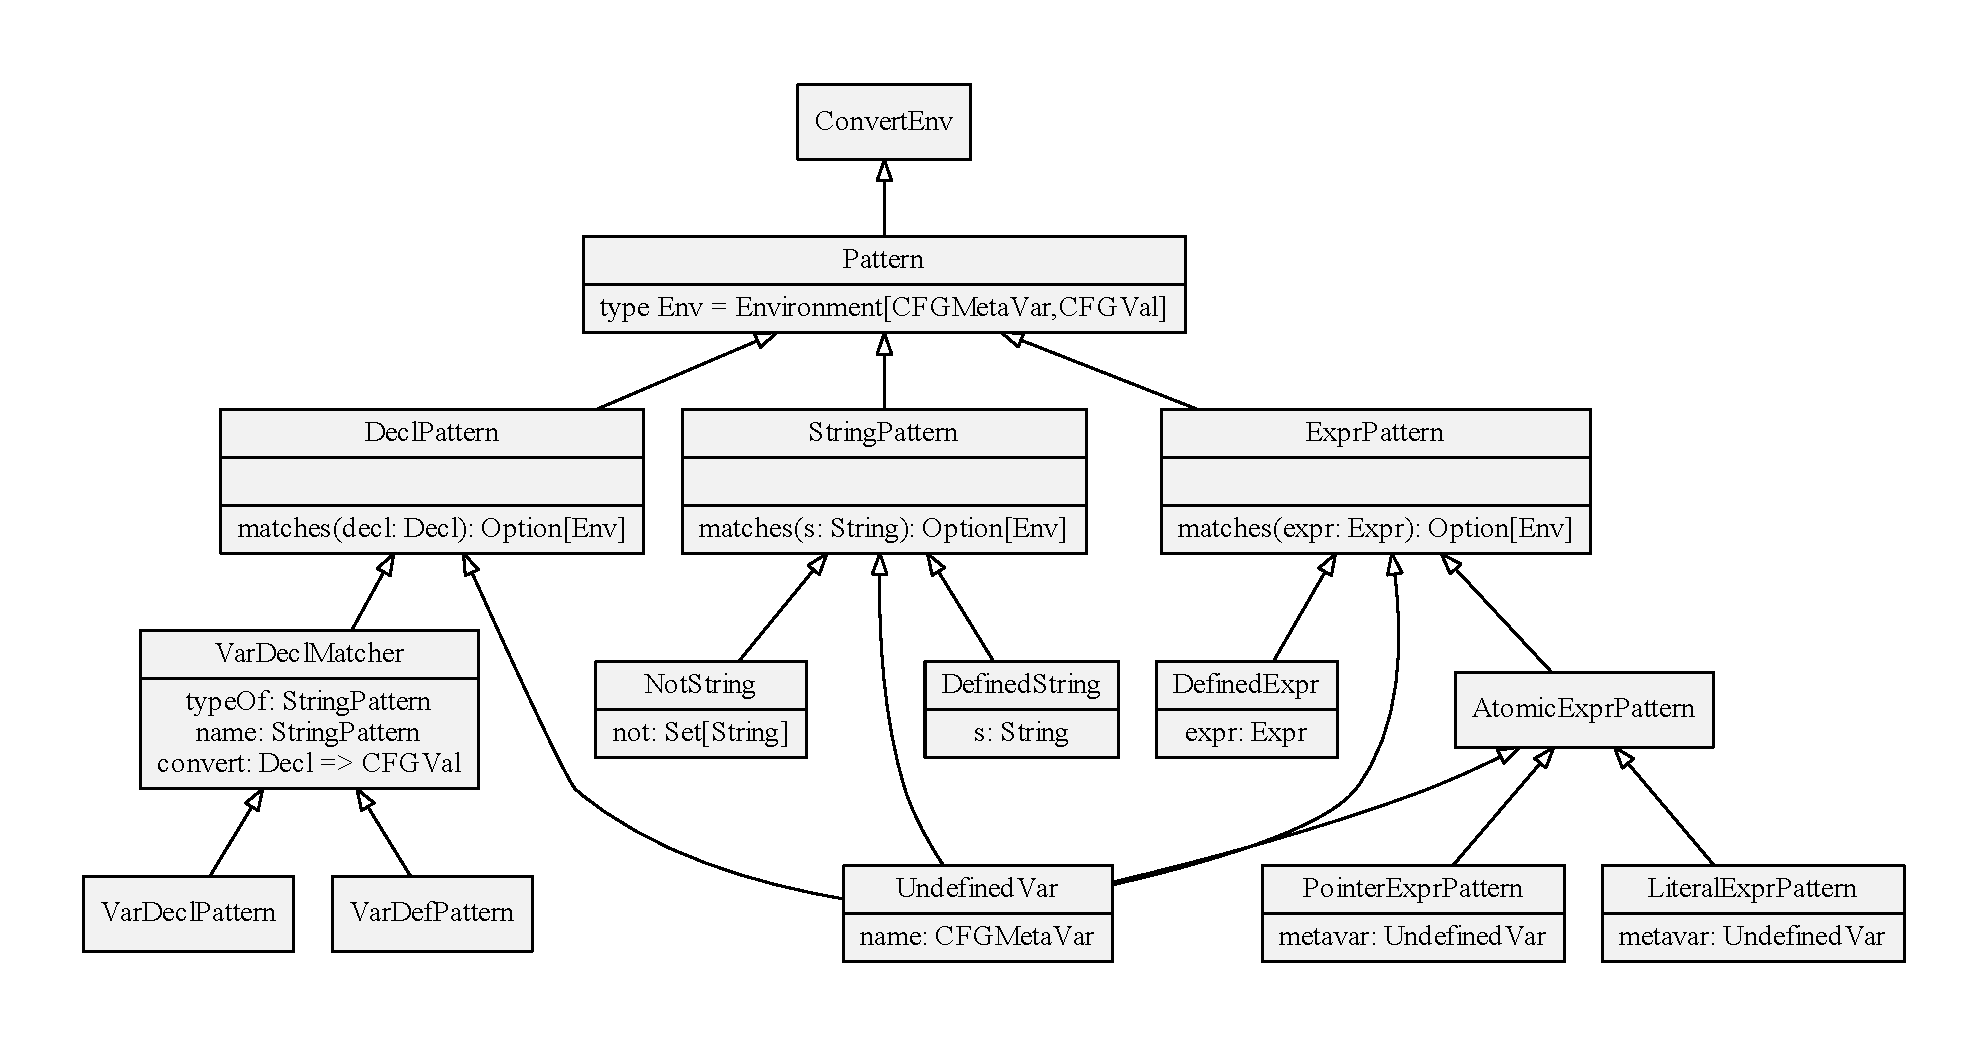
\includegraphics[scale=0.55]{data/patterns}
~\\~\\Figure III.8 - Hierarchy of the Pattern type
\end{center}

\begin{center}
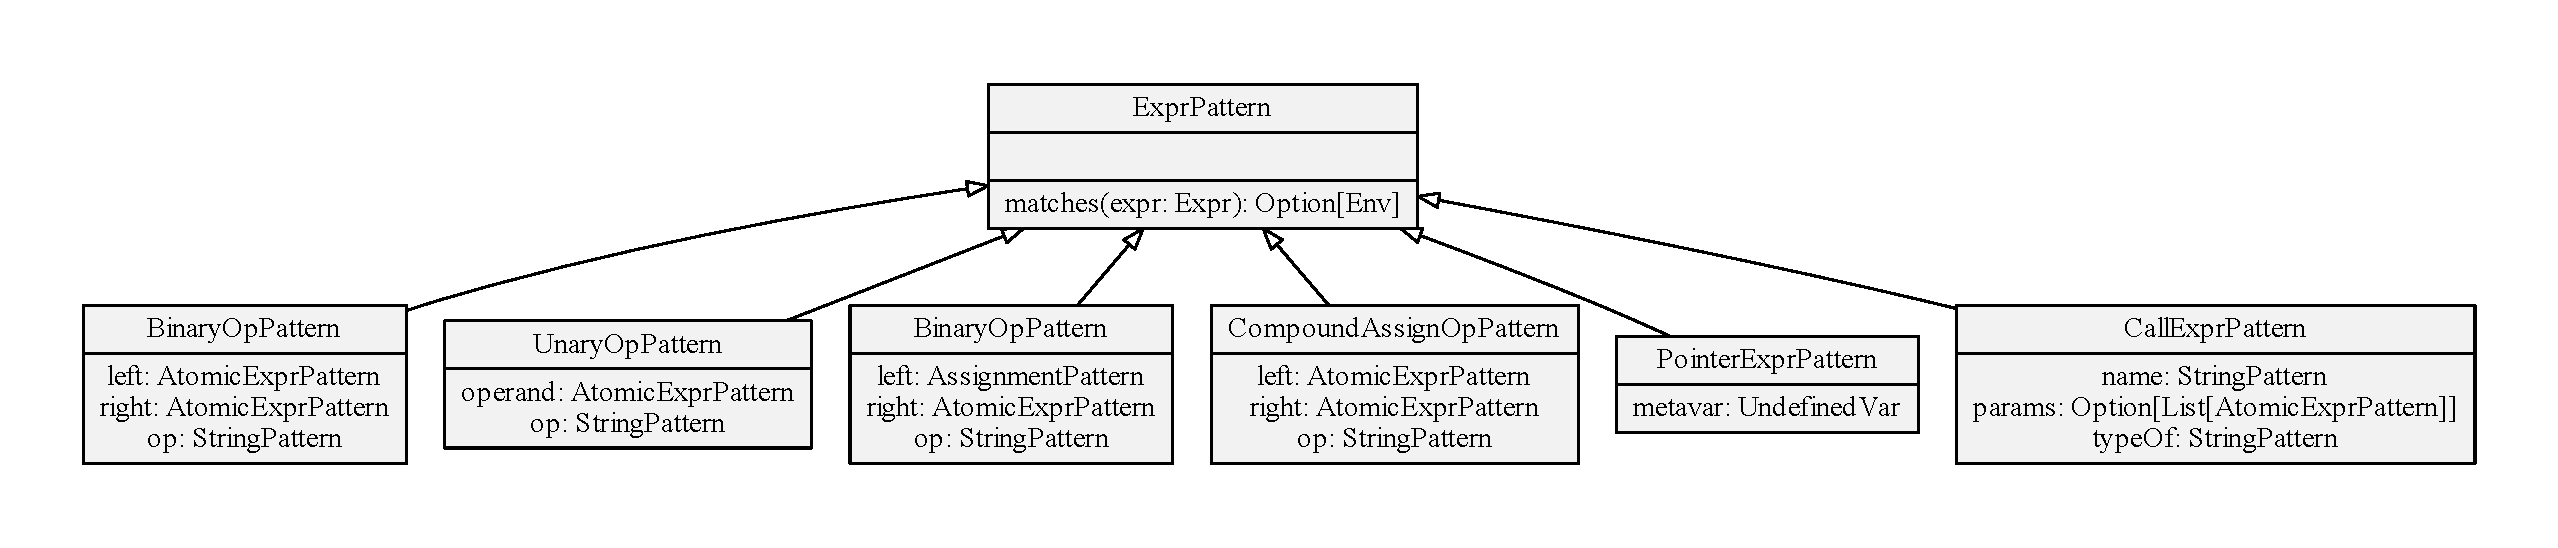
\includegraphics[scale=0.45]{data/expr_pattern}
~\\~\\Figure III.9 - Detail of all the expression patterns
\end{center}

\subsection* {Labelizers}
\paragraph{}
\hspace{4mm}Basically, our labelizers simply wrap a Pattern to add a specific semantic. Here is the list of all the labelizers, with their semantic :

\vspace{1.5mm}
\begin{itemize}
\item \textbf{IfLabelizer}, \textbf{ForLabelizer}, \textbf{WhileLabelizer}, \textbf{SwitchLabelizer}, \textbf{ExpressionLabelizer} :
all those labelizers firstly check than the node considered is of the appropriate type (respectively : If, For, While, Switch, Expression) and then if the expression
it eventually holds matches a given pattern.\vspace{1mm}
\item \textbf{VarDeclLabelizer}, \textbf{VarDefLabelizer} : match any Statement node containing a VarDecl matching a given pattern. The difference betwen those two classs is the kind of CGVal returned
in case of success (CFGDecl or CFGDef).\vspace{1mm}
\item \textbf{FindExprLabelizer} : matches any node containing at least an occurrence of a given pattern. Returns all the occurrences of the pattern in the node.\vspace{1mm}
\item \textbf{MatchesExprLabelizer} : matches any node holding an expression that exactly matches a given pattern. It returns a single value in case of success, which makes it different from FindExprLabelizer.\vspace{1mm}
\end{itemize}

\begin{center}
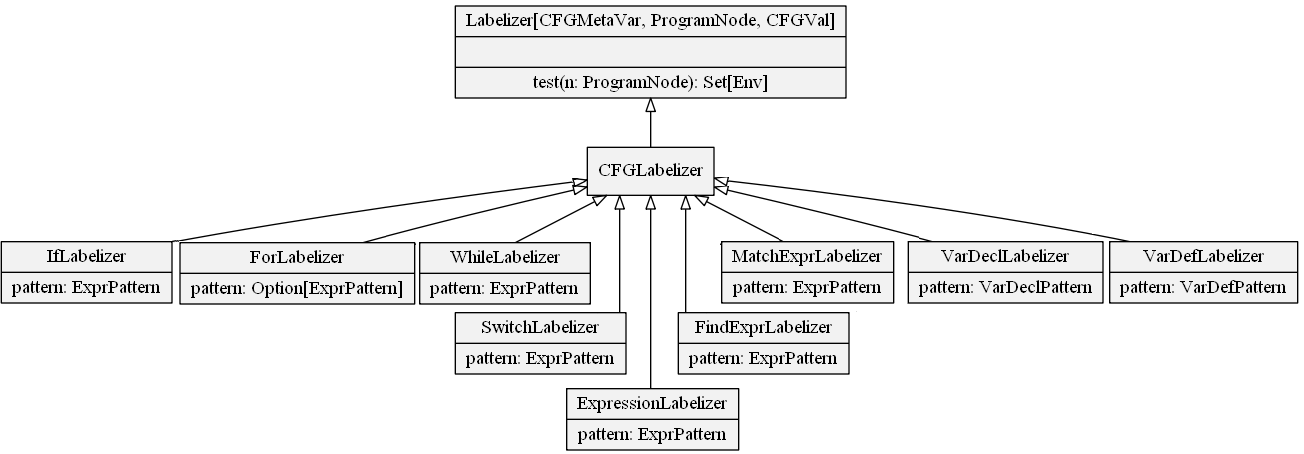
\includegraphics[scale=0.55]{data/labels.png}
~\\~\\Figure III.10 - Detail of all the labelizers we implemented
\end{center}

\end{document}
